\documentclass{article}
\usepackage[utf8]{inputenc}
\usepackage[english]{babel}
\usepackage{amsmath}
\usepackage{amssymb}
\usepackage{graphicx}

\newcommand{\lapl}{\ensuremath{\Delta}}
\newcommand{\dxy}{\ensuremath{\,\mathrm{d}x\mathrm{d}y}}

\title{Problem statement - Stage 1}
\author{Milan Hanu{\v s} and Roman Ku{\v z}el}
\date{\today}

\begin{document}
\maketitle
  
  
  
  \paragraph{Problem description:} 
  Our goal is to model the equilibrium deflection of a rectangular membrane loaded from top by a volume of arbitrary fluid. The membrane is fixed along its perimeter and is made of an arbitrary number of patches with different material having constant parameters. Deflection of the membrane in vertical direction is governed by the following equation:
$$
\nabla\cdot \bigl( t(x,y) \nabla \varphi(x,y) \bigr) - g\rho(x,y)\varphi(x,y) = p(x,y),
$$
whose terms have the following meanings and units:
\begin{center}
   \begin{tabular}{ccc}
  		$\varphi$ & unknown vertical displacement & $m$, \\
  		$t$ & tension per unit length & $N/m$,   \\
  		$\rho$ & fluid density & $kg/m^3$, \\
  		$g$ & gravitational constant & $m/s^2$, \\
  		$p$ & additional external pressure & $N/m^2$.
  \end{tabular}
\end{center}
Note that the second term on the left hand side represents the hydrostatic pressure of the fluid contained over the deflected membrane. The additional pressure $p$ may be caused e.g. by gravitational force or any other externally applied force except the hydrostatic one.\\[.2em]
  
  
 
  \paragraph{Problem Input:} $ n,h, T, g, \varrho, P $, where 
  
\begin{center}
   \begin{tabular}{ll}
  		$n$ & \ldots number of patches (same in both horizontal and vertical directions),\\
  		$h$ & \ldots uniform size of each square patch,\\
        $T$ &$= \bigcup_{j,k\in \{1,..,n\}}T_{jk}$, \\
  		$\varrho$ &$ \in \mathbb{R}^+$, \\
  		$P$ &$ \in \mathbb{R}^+$.\\
  \end{tabular}
  \end{center}

Set
\begin{center}
   \begin{tabular}{ll}
  
  		$\Omega = \bigcup_{j,k\in \{1,..,n\}} \Omega_{jk}$,   &$\Omega_{jk} = I_j \times I_k$,\\
  		& $I_k = \bigl[ (k-1)h, kh  \bigr],  \quad k=1,2, \ldots, n$,\\
        $t(x,y) = T_{jk}$ & on $\Omega_{jk}$,\\
        $\rho(x,y) = \varrho$ & on $\Omega$,\\
        $p(x,y) = P$ & on $\Omega$.\\
   \end{tabular}
  \end{center}


Boundary condition:
  $$
  \varphi(x,y) = 0, \quad (x,y)\in \partial \Omega.
  $$
  
  \paragraph{Problem output:} $\Phi$ and \texttt{time} where
 
 \begin{align*}		
    \Phi &= \sum_{j,k\in \{1,..,n\}}\Phi_{jk}, \quad \Phi_{jk}=\int_{\Omega_{jk}}\varphi(x,y)dxdy,\\
    \texttt{time}& \ldots \mbox{ running time in seconds.}
  \end{align*}
  
 \paragraph{Example} with $n = 2$:\\[.5em]
 \begin{center}
 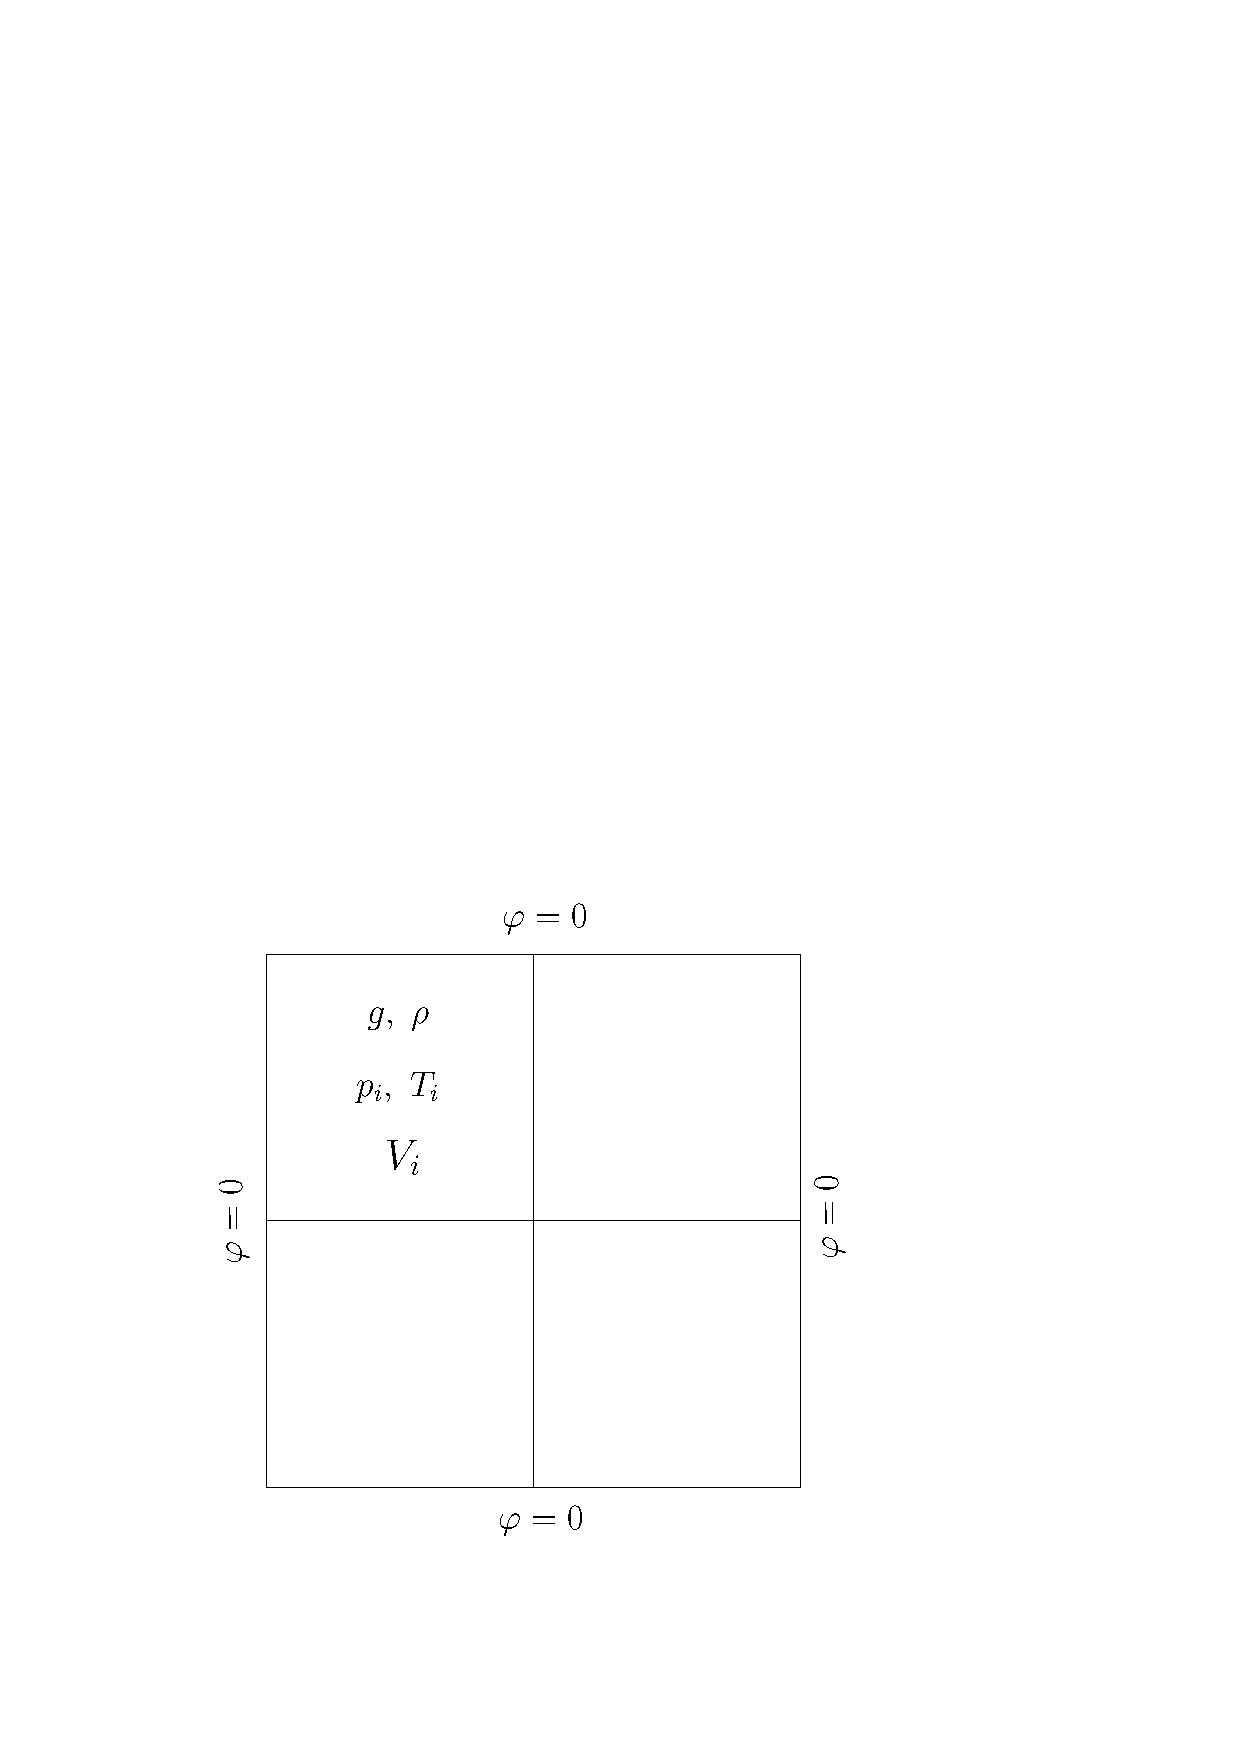
\includegraphics[scale=.6]{geometry}
 \end{center}
\end{document}
